\documentclass{article}
\usepackage[a4paper, total={6.5in, 8.5in}]{geometry}
\usepackage{graphicx}
\usepackage{booktabs}
\usepackage[label=corner]{karnaugh-map}
\usepackage{tabularray}
\usepackage{multicol}
\usepackage{multirow}
\usepackage{array}
\usepackage{hyperref}
\hypersetup{
	colorlinks=true,
	linkcolor=blue,
}
\usepackage{float}
\usepackage{caption}
\usepackage{subcaption}
\usepackage[siunitx, RPvoltages]{circuitikz}
\usetikzlibrary{calc}
\usepackage{tikz, pgfplots}
\usetikzlibrary{positioning}
\usepackage{enumitem}
\usepackage{biblatex}
\usepackage{rotating}
\usepackage{ragged2e}
%\usepackage[outputdir=../../]{minted}

{\renewcommand\fcolorbox[4][]{\textcolor{cyan}{\strut#4}}
	
	\setlength{\parskip}{1em} % Adjust the value as needed
	
	% Cover Page
	
	
	
	
	\title{CSE 306 \\
		Computer Architecture Sessional \\
		
		\vspace{5mm}
		
		\begin{figure}[h]
			\centering
			
\includegraphics[width=0.3\textwidth]{images/buet.png}
			\label{fig:enter-label}
		\end{figure}
		
		\vspace{5mm}
		Assignment-3\\
		4-bit MIPS Implementation \\
		\vspace{10mm}
		Section - A1 \\
		Group - 01 \\
		\vspace{15mm}
		\RaggedRight
		Group Members: \\
		\normalsize	{
			\centering
			\begin{enumerate}[]
				\item 2005001 - Anik Saha
				\item 2005012 - Abrar Jahin Sarker
				\item 2005013 - Al Muhit Muhtadi
				\item 2005017 - Abdullah Muhammed Amimul Ehsan
				\item 2005023 - Jaber Ahmed Deeder
			\end{enumerate}
		}
	}
	\author{}
	\date{}
	
	
	
	
	\begin{document}
		
		\maketitle
		
		
		
		
		
		% Section 1 - Amim
		
		
		\section{Introduction}
		
		This assignment  presents the design and implementation of a 4-bit MIPS (Microprocessor without Interlocked Pipeline Stages) architecture in hardware. The objective is to develop a simplified version of the MIPS architecture suitable for educational purposes, focusing on understanding fundamental concepts such as instruction formats, data paths, and control units.
		
		The 4-bit MIPS architecture is characterized by its limited data bus size of 4 bits and an address bus size of 8 bits. The design incorporates essential components such as a 4-bit ALU (Arithmetic Logic Unit), register file with temporary registers, and separate memory units for instructions and data.
		
		The instruction set of the 4-bit MIPS architecture consists of various categories, including arithmetic, logic, memory access, and control instructions. Each instruction is represented by a unique opcode and follows one of the four instruction formats: R-type, S-type, I-type, or J-type. These formats specify the arrangement of opcode, source and destination registers, immediate values, and shift amounts within a 16-bit instruction word.
		
		To facilitate the execution of instructions, the MIPS architecture utilizes two distinct memory units: instruction memory and data memory. Instruction memory is accessed through the Program Counter (PC) register, while data memory is accessed based on the provided address.
		
		Our implementation of MIPS contains these key components:
		\begin{enumerate}
			\item \textbf{Program Counter} The Program Counter (PC) is a critical component of the MIPS (Microprocessor without Interlocked Pipeline Stages) architecture, serving as a register that stores the memory address of the next instruction to be fetched and executed. Below are key points explaining the role and functionality of the Program Counter in a MIPS processor:
			
			\begin{itemize}
				
				
				
				\item \textbf{Incrementing:} After fetching an instruction from memory, the PC is automatically incremented to point to the next sequential memory address where the next instruction resides. This ensures the sequential execution of instructions in the program.
				
				\item \textbf{Branching:} The PC can be modified during program execution to implement control flow operations such as branches and jumps. Conditional branches and unconditional jumps change the PC value to redirect the flow of control to different memory addresses based on certain conditions or program requirements.
				
				\item \textbf{Jumping :} The PC holds the address of the instruction to jump in case of jump instructions.
				
				
				
				\item \textbf{Reset:} Upon system startup or reset, the PC is typically initialized to a predefined memory address, usually the beginning of the program or the operating system kernel, to start program execution from a known starting point.
			\end{itemize}
			
			In summary, the Program Counter (PC) in a MIPS processor is responsible for maintaining the address of the next instruction to be executed, facilitating sequential instruction execution, controlling program flow through branches and jumps, and participating in lots of other mechanisms. It is a critical component of the MIPS architecture, enabling efficient and orderly execution of programs.
			\item \textbf{Instruction Memory}
			
			Instruction Memory is a component of the MIPS processor responsible for storing machine instructions that the processor fetches and executes during program execution.Below are key points explaining the role and functionality of Instruction Memory in a MIPS processor:
			
			\begin{itemize}
				
				
				
				\item \textbf{Purpose:} The primary purpose of Instruction Memory is to hold the program instructions that the processor needs to execute. These instructions are fetched sequentially from memory and transferred to the instruction pipeline for decoding and execution.
				
				\item \textbf{Organization:} Instruction Memory is organized as a sequential array of memory cells or locations, each containing one instruction word. In a typical MIPS architecture, each instruction word is 32 bits (4 bytes) long.Here,our instructions are 16 bits(2 Bytes) long.
				
				\item \textbf{Access:} During the fetch stage of the instruction pipeline, the processor retrieves the instruction at the current Program Counter (PC) address from the Instruction Memory. The fetched instruction is then decoded and executed in subsequent stages of the pipeline.
				
				
				
				\item \textbf{Addressing:} Instruction Memory is accessed using memory addresses provided by the Program Counter (PC) register. The PC holds the address of the next instruction to be fetched, and this address is used to access the corresponding instruction in memory.
				
				\item \textbf{Performance Considerations:} Efficient access to Instruction Memory is critical for overall processor performance. Techniques such as prefetching, branch prediction, and cache optimization may be employed to enhance instruction fetch efficiency and reduce stalls in the pipeline.
				
				\item \textbf{Instruction Alignment:} In MIPS architectures, instructions are typically aligned in memory, meaning they start at addresses that are multiples of their size (e.g., 4-byte aligned for 32-bit instructions or 2-byte aligned for 16-bit instructions). This alignment ensures efficient memory access and simplifies instruction fetching.
			\end{itemize}
			
			In summary, Instruction Memory in a MIPS architecture serves as the storage space for program instructions, facilitating their sequential retrieval and execution by the processor. It plays a crucial role in overall processor performance and is accessed using memory addresses provided by the Program Counter.
			\item \textbf{Register File : }
			The register file is a crucial component of the MIPS (Microprocessor without Interlocked Pipeline Stages) architecture, providing storage space for operands, intermediate results, and other data during program execution. Below are key points explaining the register file in the context of the 4-bit MIPS architecture:
			
			\begin{itemize}
				
				\item \textbf{Size and Composition:} The register file consists of several 4-bit registers, each capable of storing values from 0 to 15 ($2^4 - 1$). Specifically, it includes the following temporary registers:
				\begin{itemize}
					\item \$zero: A special register that always holds the value zero.
					\item \$t0,\$ t1,\$ t2,\$ t3,\$ t4: Temporary registers used for general-purpose storage and computation.
				\end{itemize}
				
				\item \textbf{Purpose:} The register file serves as a fast and efficient storage location for data that the processor needs to access frequently during program execution. It allows for quick retrieval and manipulation of operands for arithmetic, logic, and data movement operations.
				
				\item \textbf{Usage in Assembly Code:} The assembly code provided to simulate the MIPS design will utilize the above-mentioned registers for data manipulation. Instructions in the code will specify these registers as the source and destination operands for various operations.
				
				\item \textbf{Access and Operation:} During program execution, the processor accesses the register file to read operand values and store results. The control unit coordinates the read and write operations to the register file based on the instructions being executed.
				
				\item \textbf{Benefits:} Using registers for temporary storage offers several advantages, including fast access times, efficient data movement, and support for parallel execution of instructions.
			\end{itemize}
			
			In summary, the register file in the 4-bit MIPS architecture provides storage space for operands and intermediate results, facilitating efficient data manipulation and computation during program execution.
			
			
			
			\item \textbf{ALU : }
			The Arithmetic Logic Unit (ALU) is a crucial component of the MIPS (Microprocessor without Interlocked Pipeline Stages) architecture. Below are key points explaining the role and functionality of the ALU in a MIPS processor:
			
			\begin{itemize}
				
				
				
				\item \textbf{Functionality:} The ALU executes arithmetic operations such as addition, subtraction, multiplication, and division, as well as logical operations such as AND, OR, XOR, and shift operations.
				
				\item \textbf{Data Width:} In the context of the MIPS architecture, the ALU typically operates on data of fixed width. For example, in a 32-bit MIPS processor, the ALU handles 32-bit data.Here,Our ALU handles 4 bit data.
				
				\item \textbf{Inputs:} The ALU receives input operands from registers or immediate values specified in instructions. These operands are passed to the ALU for processing.
				
				\item \textbf{Operation Selection:} The operation to be performed by the ALU is determined by the opcode field of the instruction being executed. The opcode specifies the type of operation to be executed (e.g., addition, subtraction, logical AND, logical OR).
				
				\item \textbf{Output:} After performing the specified operation, the ALU produces a result, which is then stored in a destination register or used as input for subsequent instructions.
				
				\item \textbf{Flags:} In addition to the result, the ALU may set status flags based on the outcome of the operation. Common flags include zero flag (indicating if the result is zero), carry flag (indicating if a carry occurred in arithmetic operations), and overflow flag (indicating if the result exceeds the representable range).Zero flag is necessary for branching.
				
				\item \textbf{Speed and Efficiency:} The ALU is designed to execute operations quickly and efficiently, as it is a critical component of the processor responsible for performing the bulk of the computational tasks.
				
				
			\end{itemize}
			
			In summary, the Arithmetic Logic Unit (ALU) in the MIPS architecture is responsible for executing arithmetic and logical operations on data. It plays a crucial role in performing computational tasks and manipulating data within the processor.
			
			\item \textbf{Data Memory : }
			Data Memory, also known as the Data Cache or Data Cache Memory, is a fundamental component of the MIPS (Microprocessor without Interlocked Pipeline Stages) architecture.  It serves as the main storage space for variables, arrays, and other data structures.Below are key points explaining the role and functionality of Data Memory in a MIPS processor:
			
			\begin{itemize}
				
				
				
				\item \textbf{Purpose:} The primary purpose of Data Memory is to hold data that the processor reads from or writes to during program execution. This includes both input data and intermediate results generated by the processor.
				
				\item \textbf{Organization:} Data Memory is organized as a sequential array of memory cells or locations, each capable of storing one data word. The size of each data word depends on the architecture but is typically 32 bits (4 bytes) in a MIPS processor.Here,the size of each word is 4 bits.
				
				\item \textbf{Access:} During program execution, the processor accesses Data Memory to read input data or store computed results. Data is read from or written to memory using memory addresses provided by the instruction being executed.
				
				\item \textbf{Addressing:} Data Memory is accessed using memory addresses provided by the instruction being executed. The memory address specifies the location in Data Memory from which data is to be read or written.
				
				
				
				
			\end{itemize}
			
			In summary, Data Memory in the MIPS architecture serves as the primary storage space for data manipulated by the processor during program execution. It plays a crucial role in storing input data, intermediate results, and program variables, and efficient access to Data Memory is essential for overall processor performance.
			
			
			\item \textbf{Control Unit : }
			The control unit in a MIPS (Microprocessor without Interlocked Pipeline Stages) processor is a vital component responsible for generating control signals that coordinate the execution of instructions and manage data flow within the processor. Below are key points explaining the control unit in the context of the provided MIPS instructions:
			
			\begin{itemize}
				
				\item \textbf{Functionality:} The control unit interprets the opcode of each instruction and generates the necessary control signals to coordinate the operation of other components in the processor, such as the ALU, register file, and data memory.Multiplexers receives their control bits from control unit and provides the expected bits.
				
				\item \textbf{Instruction Categories:} The provided instructions can be categorized into arithmetic, logic, memory access, and control instructions. Each instruction category may require specific control signals to be generated by the control unit.
				
				\item \textbf{Control Signals:} Based on the opcode of each instruction, the control unit generates control signals to perform various tasks, including selecting the appropriate operation for the ALU, enabling data transfers between the register file and data memory, and managing program flow based on conditional branches and unconditional jumps.
				
				\item \textbf{Microprogramming:} In the described MIPS architecture, the control unit should be micro-programmed. This means that the control signals associated with different operations are stored in a special memory unit, such as EEPROM, as control words. The control unit fetches these control words based on the opcode of the current instruction being executed.
				
				\item \textbf{Integration with Other Components:} The control unit interacts closely with other components of the processor, such as the ALU, register file, program counter (PC), and data memory. It coordinates the timing and sequencing of operations to ensure correct execution of instructions.
			\end{itemize}
			
			In summary, the control unit in the MIPS architecture plays a crucial role in coordinating the execution of instructions by generating appropriate control signals, interpreting opcodes, and managing data flow within the processor.
			
		\end{enumerate}
		
		Apart from these,we needed 6 multiplexers.Multiplexers are used to send the correct bits to the next unit.These multiplexers are controlled by control unit.\\
		
		Adders were required to calculate address of the next instruction where Program counter will point to.Two adders were needed here.
		
		
		
		
		\newpage
		
		% Section 2 - Muhit
		
		
		
		\section{Instruction Set}
		\begin{table}[h]
			\centering
			\begin{tabular}{|c|c|c|c|c|}
				\hline
				Instruction ID & Op code & Category & Type & Instruction\\
				\hline
				A & 1111 & Arithmetic & R & add\\
				\hline
				B & 1011 & Arithmetic & I & addi\\
				\hline
				C & 1101 & Arithmetic & R & sub\\
				\hline
				D & 0001 & Arithmetic & I & subi\\
				\hline
				E & 1000 & Logic & R & and\\
				\hline
				F & 0111 & Logic & I & andi\\
				\hline
				G & 1100 & Logic & R & or\\
				\hline
				H & 1110 & Logic & I & ori\\
				\hline
				I & 0101 & Logic & R & sll\\
				\hline
				J & 0000 & Logic & R & srl\\
				\hline
				K & 0011 & Logic & R & nor\\
				\hline
				L & 0100 & Memory & I & sw\\
				\hline
				M & 0110 & Memory & I & lw\\
				\hline
				N & 0010 & Control-conditional & I & beq\\
				\hline
				O & 1001 & Control-conditional & I & bneq\\
				\hline
				P & 1010 & Control-unconditional & J & j\\
				\hline
			\end{tabular}
			\caption{Instruction Set}
			\label{tab:table1}
		\end{table}
		
		
		
		
		\newpage
		
		% Section 3 - Jahin and Jaber
		
		
		
		\section{Complete Block diagram of a 4-bit MIPS processor}
		
		\begin{figure}[h]
			\centering
			\includegraphics[scale=0.3]{images/block3.png}
			\caption{Complete Block Diagram}
			\label{fig:enter-label}
		\end{figure}
		
		
		\newpage
		
		% Section 4 - Jahin and Jaber
		
		
		
		\section{\large{Block diagrams of the main components}}
		
		\subsection{PC Register}
		
		\begin{figure}[h]
			\centering
			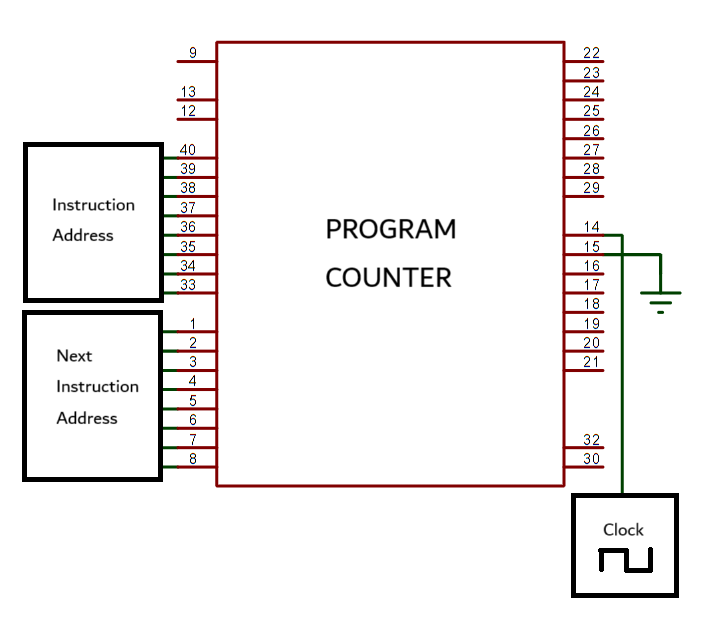
\includegraphics[scale=0.9]{images/pc.png}
			\caption{PC Register}
			\label{fig:enter-label}
		\end{figure}
		
		\newpage
		
		\subsection{Instruction Memory}
		
		\begin{figure}[h]
			\centering
			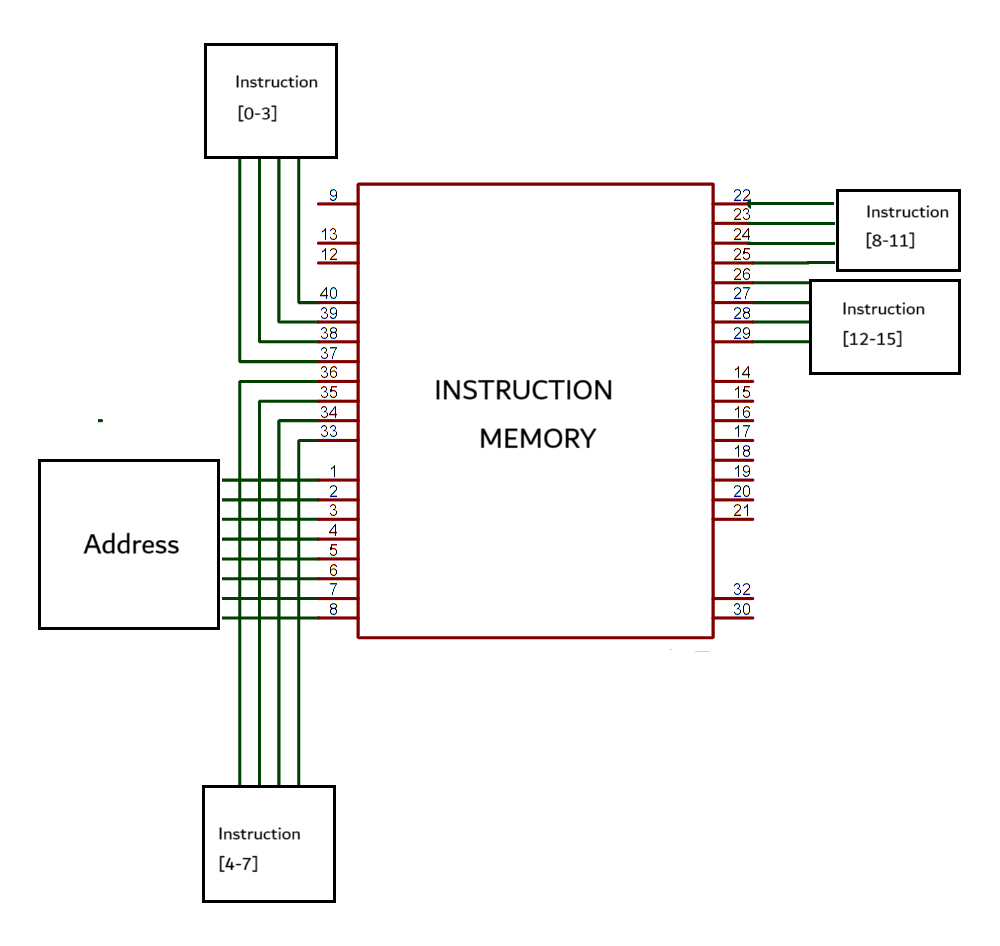
\includegraphics[scale=0.9]{images/im.png}
			\caption{Instruction Memory}
			\label{fig:enter-label}
		\end{figure}
		
		\newpage
		
		\subsection{Register Files}
		
		\begin{figure}[h]
			\centering
			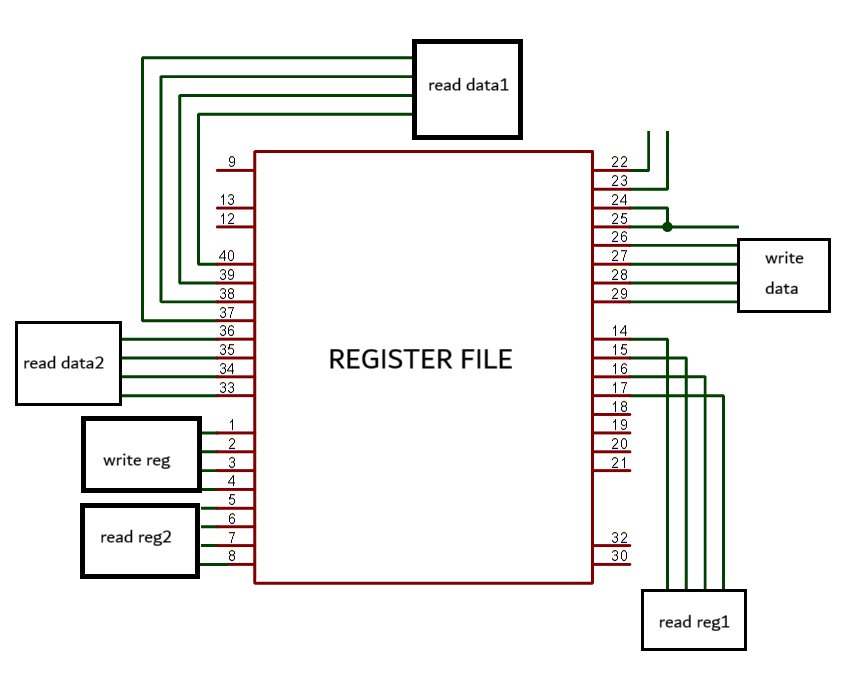
\includegraphics[scale=0.9]{images/rf.png}
			\caption{Register Files}
			\label{fig:enter-label}
		\end{figure}
		
		\newpage
		
		\subsection{Arithmetic and Logic Unit}
		
		\begin{figure}[h]
			\centering
			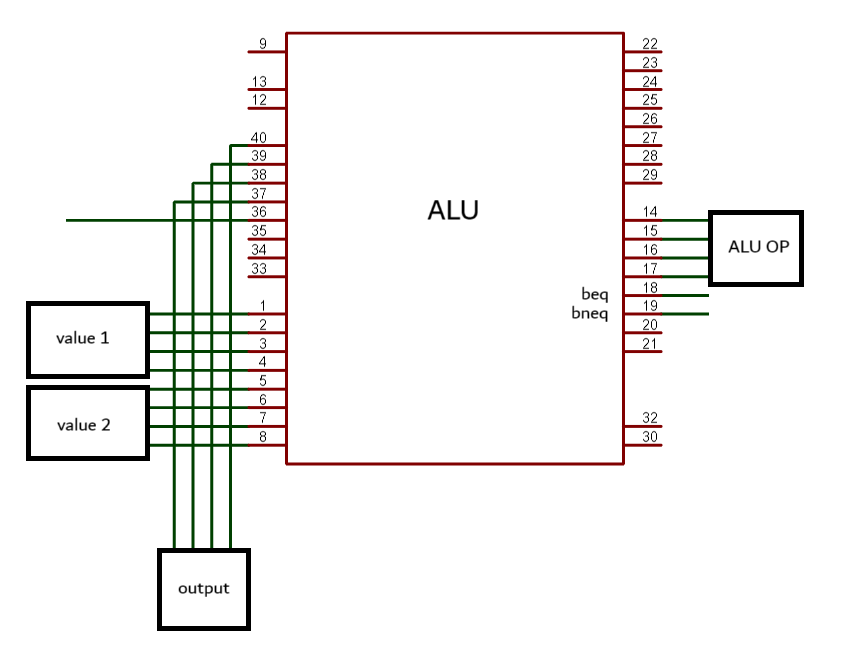
\includegraphics[scale=0.9]{images/alu.png}
			\caption{Arithmetic and Logic Unit}
			\label{fig:enter-label}
		\end{figure}
		
		\newpage
		
		\subsection{Data Memory}
		
		\begin{figure}[h]
			\centering
			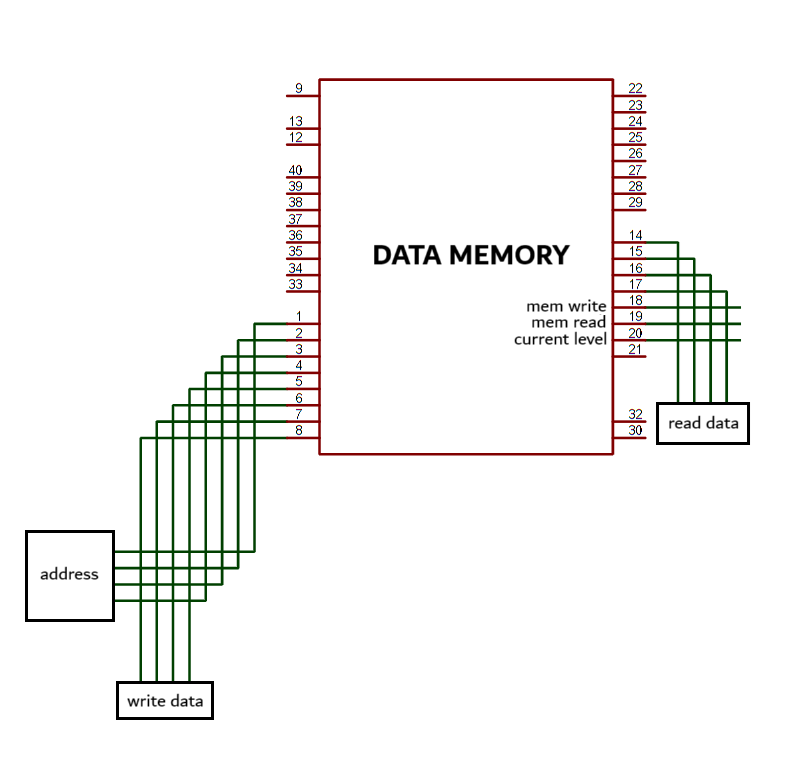
\includegraphics[scale=0.9]{images/dm.png}
			\caption{Data Memory}
			\label{fig:enter-label}
		\end{figure}
		
		\newpage
		
		% Section 5 - Anik
		
		
		\section{\large{Approach to implement the push and pop instructions}}
		
		According to the specification, following are the formats of  push and pop instructions which need to be incorporated into our design.
		
		\begin{table}[H]
			\centering
			\begin{tabular}{|c|c|}
				\hline
				Instruction & Description \\
				\hline
				\textbf{push \$t0} & mem[\textbf{\$sp}] = \textbf{\$t0}    \\
				\hline
				\textbf{push 3(\$t0)} & mem[\textbf{\$sp}] = mem[\textbf{\$t0}+3]  \\
				\hline
				\textbf{pop \$t0} & \textbf{\$t0} = mem[\textbf{\$sp}] \\
				\hline
			\end{tabular}
			\caption{Push and Pop Instruction Formats}
			\label{tab:my_label}
		\end{table}
		
		The salient idea behind implementing each of the operations is that these instructions can be viewed as compound instructions consisting of two or more simple instructions that are directly supported by our design. Let us explore the details of the approach for each of them.
		
		\begin{enumerate}
			
			% 1
			
			\item  \textbf{Register to Stack: } The first instruction refers to pushing the value of a particular register to the stack. The format is \textbf{push \hspace{.5mm} $<register\_name>$}
			
			\textbf{Example:} 
			
			%\begin{minted}{gas}
				push \$t0
			%\end{minted}
			
			This instruction may be viewed as comprising the following steps:
			
			\begin{enumerate}
				\item Decrease the value of \textbf{\$sp} by one to indicate that a new value is pushed onto the stack
				
				\item Store the value at the register \textbf{\$t0} to the topmost position of the stack. The topmost position is denoted by the address pointed to by the register \textbf{\$sp}.
				
			\end{enumerate}
			
			It is easy to see that the corresponding pair of assembly instructions for the above-mentioned steps are:
			
			%\begin{minted}{gas}
				subi \$sp, \$sp, 1
				sw \$t0, 0(\$sp) 
			%\end{minted}
			
			Note that, since this instruction is broken down into 2 simple instruction, it requires 2 clock cycles to execute.
			
			\vspace{3mm}
			
			\item  \textbf{Memory to Stack: } The second instruction refers to pushing the value of a particular memory location to the stack. The format is \textbf{push \hspace{.5mm} $<memory_address>$}
			
			\textbf{Example:} 
			
			%\begin{minted}{gas}
				push 3(\$t0)
			%\end{minted}
			
			To accomplish this instruction, we are using a hidden register which we have named as \$hd.
			
			This instruction may be viewed as comprising the following steps:
			
			\begin{enumerate}
				\item Decrease the value of \textbf{\$sp} by one to indicate that a new value is pushed onto the stack
				
				\item Load the value at the topmost position of the stack to the hidden register \textbf{\$hd}. The topmost position is denoted by the address pointed to by the register \textbf{\$sp}
				
				\item Store the value at the hidden register \textbf{\$hd} to the topmost position of the stack. The topmost position is denoted by the address pointed to by the register \textbf{\$sp}.
				
			\end{enumerate}
			
			It is easy to see that the corresponding trio of assembly instructions for the above-mentioned steps are:
			
			%\begin{minted}{gas}
				subi \$sp, \$sp, 1
				lw \$hd, 3(\$t0)
				sw \$hd, 0(\$sp) 
			%\end{minted}
			
			Note that, since this instruction is broken down into 3 simple instruction, it requires 3 clock cycles to execute.
			
			\vspace{3mm}
			
			
			
			% 3
			
			\item \textbf{Stack to Register: } The third instruction refers to popping the topmost value on the stack and loading that value into a particular register. The format is \textbf{pop \hspace{.5mm} $<register\_name>$}
			
			\textbf{Example:} 
			
			%\begin{minted}{gas}
				pop \$t0
			%\end{minted}
			
			This instruction may be viewed as comprising the following steps:
			
			\begin{enumerate}
				\item Load the value at the topmost position of the stack to the register \textbf{\$t0}. The topmost position is denoted by the address pointed to by the register \textbf{\$sp}
				
				\item Increase the value of \textbf{\$sp} by one to indicate that a value is popped from the stack.
				
			\end{enumerate}
			
			It is easy to see that the corresponding pair of assembly instructions for the above-mentioned steps are:
			
			%\begin{minted}{gas}
				lw \$t0, 0(\$sp) 
				addi \$sp, \$sp, 1
			%\end{minted}
			
			Note that, since this instruction is broken down into 2 simple instruction, it requires 2 clock cycles to execute.
			
			
		\end{enumerate}
		
		
		\newpage
		
		
		% Section 6 - Amim
		
		
		\section{ICs used with their count}
		\begin{table}[h]
			\centering
			\begin{tabular}{|c|c|c|}
				\hline
				\textbf{IC category} & \textbf{IC Number} & \textbf{Count}  \\
				\hline
				{}& ATMEGA32A & 6\\
				\hline
				$ 2\times 1 Multiplexer$ & 74157 & 6\\
				\hline
				4 bit Adder & 7483 & 2\\
				\hline
				\multicolumn{2}{|c|}{Total} & 14
				\\
				\hline
			\end{tabular}
			\caption{IC Count}
			\label{ICs used with their count}
		\end{table}
		
		
		\newpage
		
		
		% Section 7 - Anik
		
		
		\section{Discussion}
		
		
		This assignment on the implementation of a 4-bit-MIPS processor significantly helped us bridge through the chasms of our knowledge of Computer Architecture enabling us to visualize the entirety of the whole workflow from writing a piece of code in a fancy editor to carrying out bit-level instructions in real hardware. Although a shade of abstraction becomes prevalent owing to the use of microcontrollers in the design, the underlying ideas remain all the same and the stream of actions replicate the actual process to a considerable extent.
		
		Prior to designing the circuitry, we needed to have developed a codebase for parsing an assembly file written in MIPS assembly language to machine-readable code. The codebase, written in python, parses the given assembly file, reports errors(if any), and converts it to a machine code as per the given instruction set corresponding to our assigned permutation. Since the control bits have been micro-programmed, it also generates a hard-coded array of binary strings representing the control bits for different opcodes. These binary arrays for control bits and instructions are in turn used in the software simulation.
		
		To perform the software simulation, we preferred to resort to Proteus since we used the microcontroller named ATmega32 in our design. To ensure that the use of microcontroller does not trivilalize our design, we used separate ATmega's for each of the stages of our MIPS processor. One additional ATmega was used to serve as the Control Unit. Furthermore, we used multiplexers and 4-bit adders for the calculation of the next value of program counter. For showing the 'write-back-value' of the current instruction, we connected 4 LEDs to the corresponsing pins of the relevant ATmega32. To trace the workflow of the jump and branch instructions, we also connected 4 LEDs showing the lower 4 bits of the program counter(assuming that the number of instructions will not exceed 16, for demonstration purposes).
		
		Then comes the hardware implementation filled with multi-dimensional challenges. To parallelize our activities, we kept building the two halves of the circuit simultaneously and merged them afterwards. Extensive care was taken to avoid wire-crossings so that the circuit looks cleaner. Wires were meticulously inserted into breadboard pins so that they don't touch other adjacent wires and thereby cause short circuits. Since ATmega32 is highly sensitive to the provided voltage and a sudden uprise of voltage may rupture the internal circuitry, preventing unintended shorting connections was of paramount importance. After the circuit was built, the hex files were burnt into the microcontrollers with the help of 'Extreme Burner'. Although 5 of them need to be burnt only once, the ATmega acting as the Instruction Memory need to be burnt every time every time the intended assembly code changes. The corresponding machine code is generated for the given assembly code and is then loaded onto that microcontroller.
		
		To assess the outputs, we speculated the 'write-back-value's of each instruction beforehand and later matched them with the outputs in LEDs. In case of branch and jump instructions, we also kept an eye on the program counter LEDs to detect whether the program control switches to the appropriate place. 
		
		One particular hurdle we needed to battle against was themechanical bouncing of push button switch that we used to manually trigger clock edges. To introduce debouncing, we added a delay of 500ms right after the detection of a clock edge so that subsequent unintended bouncing do not cause the program counter to leap forward.
		
		
		In a nutshell, this implementation helped us gain invaluable pieces of experience that will guide us through further explorations in the coming days. We hope to explore pipelining and other optimization techniques in future to widen our understanding of processor design.
		
		
		
		
		\newpage
		
		% Section 8 - Anik
		
		\section{Contribution of Each Member}
		
		
		
		\subsection{Software Simulation}
		
		
		
		\begin{table}[h]
			\centering
			\begin{tabular}{|c|c|m{10cm}|}
				\hline
				Student ID & Surname & Contribution \\ 
				\hline
				2005001    & Anik    & Developed the python codebase for a MIPS assembler, jointly prepared the code for the microcontroller in Control Unit    \\ 
				\hline
				2005012    & Jahin   & Prepared the code for the microcontroller in Data Memory \\ 
				\hline
				2005013    & Muhit   & Prepared the code for the microcontroller in ALU  \\ 
				\hline
				2005017    & Amim    &  Prepared the code for the microcontroller in Register Files, jointly prepared the code for the microcontroller in Control Unit    \\ 
				\hline
				2005023    & Jaber   &  Prepared the code for the microcontroller in PC Register \\ 
				\hline
			\end{tabular}
		\end{table}
		
		\subsection{Hardware Implementation}
		
		
		
		\begin{table}[h]
			\centering
			\begin{tabular}{|c|c|m{10cm}|}
				\hline
				Student ID & Surname & Contribution \\ 
				\hline
				2005001    & Anik    & Jointly implemented Register Files, ALU, Data Memory    \\ 
				\hline
				2005012    & Jahin   & Jointly implemented PC Register, Instruction Memory, Control Unit  \\ 
				\hline
				2005013    & Muhit   & Jointly implemented PC Register, Instruction Memory, Control Unit     \\ 
				\hline
				2005017    & Amim    &  Jointly implemented Register Files, ALU, Data Memory    \\ \hline
				2005023    & Jaber   &  Jointly implemented PC Register, Instruction Memory, Control Unit     \\ 
				\hline
			\end{tabular}
		\end{table}
		
		
		\subsection{Verification and Testing}
		
		
		\begin{table}[h]
			\centering
			\begin{tabular}{|c|c|m{10cm}|}
				\hline
				Student ID & Surname & Contribution \\ 
				\hline
				2005001    & Anik    &  Jointly generated extensive testcases for simulation and performed relevant debugging in hardware \\ 
				\hline
				2005012    & Jahin   &  Verified the procedure for implementing push and pop instructions and the control bits for micro-programming into Control Unit \\ 
				\hline
				2005013    & Muhit   &  Jointly generated extensive testcases for simulation and performed relevant debugging in hardware \\ 
				\hline
				2005017    & Amim    & Jointly generated extensive testcases for simulation and performed relevant debugging in hardware \\ 
				\hline
				2005023    & Jaber   & Tested and debugged the assembler codebase and assisted in hardware testing \\ 
				\hline
			\end{tabular}
		\end{table}
		
		
	\end{document}
	
